\documentclass[10pt]{article}
\usepackage[utf8]{inputenc}
\usepackage[T1]{fontenc}
\usepackage{amsmath}
\usepackage{amsfonts}
\usepackage{amssymb}
\usepackage[version=4]{mhchem}
\usepackage{stmaryrd}
\usepackage{graphicx}
\usepackage[export]{adjustbox}
\graphicspath{ {./images/} }

\begin{document}
\section*{Math 141 Tutorial 7 Solutions}
\section*{Main problems}
\begin{enumerate}
  \item For the following problem compute the area enclosed by the given functions in the specified region:\\
(a) between $y=x-1$ and $y=x^{2}-x-2$\\
(b) between $y=\cos (2 x)$ and $y=\sin (x)$ for $\frac{-\pi}{2} \leq x \leq \frac{3 \pi}{2}$\\
(c) between $x=y^{2}-4 y$ and $x=2 y-y^{2}$\\
(d) between $y=e^{x}$ and $y=e^{5 x}$ for $-2 \leq x \leq 1$
\end{enumerate}

\section*{Solutions:}
(a) In order to find the enclosed area, we first determine where the curves $y=x-1$ and $y=x^{2}-x-2$ intersect. To this end, we set

$$
x-1=x^{2}-x-2 \Longleftrightarrow x^{2}-2 x-1=0
$$

The solutions to this problem are $\frac{1}{2}(2 \pm \sqrt{8})=1 \pm \sqrt{2}$.\\
Hence, the region in question is contained between $x=1-\sqrt{2}$ and $x=1+\sqrt{2}$. In this interval, the function $x-1$ will be above $x^{2}-2 x-2$ (recall from differential calculus that this can be seen by simply verifying the value of each function at any value between $1-\sqrt{2}$ and $1+\sqrt{2}$ ). The area between the curves is therefore

$$
\begin{aligned}
\int_{1-\sqrt{2}}^{1+\sqrt{2}}\left((x-1)-\left(x^{2}-2 x-1\right)\right) \mathrm{d} x & =\int_{1-\sqrt{2}}^{1+\sqrt{2}}\left(-x^{2}+3 x\right) \mathrm{d} x \\
& =-\frac{x^{3}}{3}+\left.\frac{3 x^{2}}{2}\right|_{1-\sqrt{2}} ^{1+\sqrt{2}}=\frac{8 \sqrt{2}}{3}
\end{aligned}
$$

(b) Once, again, we first find the intersection of the curves. Since $\cos (2 x)=1-2 \sin ^{2}(x)$, we see that

$$
\cos (2 x)=\sin (x) \Longleftrightarrow 1-2 \sin ^{2}(x)=\sin (x) \Longleftrightarrow 2 \sin ^{2}(x)+\sin (x)-1=0
$$

Factorizing, we obtain

$$
(2 \sin (x)-1)(\sin (x)+1)=0
$$

Hence, either $\sin (x)=1 / 2$ or $\sin (x)=-1$. Since we are in the interval $[-\pi / 2,3 \pi / 2]$, the solutions of $\sin (x)=1 / 2$ are $\pi / 6$ and $5 \pi / 6$ while the solutions of $\sin (x)=-1$ are $-\pi / 2$ and $3 \pi / 2$.\\
By plugging in an appropriate value, we can verify that

\begin{itemize}
  \item $\cos (2 x) \geq \sin (x)$ on $[-\pi / 2, \pi / 6]$
  \item $\cos (2 x) \leq \sin (x)$ on $[\pi / 6,5 \pi / 6]$
  \item $\cos (2 x) \geq \sin (x)$ on $[5 \pi / 6,3 \pi / 2]$
\end{itemize}

The area between the curves is therefore

$$
\begin{aligned}
& \int_{-\pi / 2}^{\pi / 6}(\cos (2 x)-\sin (x)) \mathrm{d} x+\int_{\pi / 6}^{5 \pi / 6}(\sin (x)-\cos (2 x)) \mathrm{d} x+\int_{5 \pi / 6}^{3 \pi / 2}(\cos (2 x)-\sin (x)) \mathrm{d} x \\
& =\left[-\frac{1}{2} \sin (2 x)+\cos (x)\right]_{-\pi / 2}^{\pi / 6}+\left[-\cos (x)-\frac{1}{2} \sin (2 x)\right]_{\pi / 6}^{5 \pi / 6}+\left[-\frac{1}{2} \sin (2 x)+\cos (x)\right]_{5 \pi / 6}^{3 \pi / 2} \\
& =\frac{3 \sqrt{3}}{4}+\frac{3 \sqrt{3}}{2}+\frac{3 \sqrt{3}}{4}=3 \sqrt{3}
\end{aligned}
$$

(c) between $x=y^{2}-4 y$ and $x=2 y-y^{2}$

We find the value of $y$ such that $y^{2}-4 y=2 y-y^{2}$. Rearranging, we have instead the equation $2 y^{2}-6 y=2 y(y-3)=0$. The solutions are $y=0$ or $y=3$. In this interval, we notice that $y^{2}-4 y \leq 2 y-y^{2}$. Hence, the area between the curves is

$$
\int_{0}^{3}\left(\left(2 y-y^{2}\right)-\left(y^{2}-4 y\right)\right) \mathrm{d} y=\int_{0}^{3}\left(6 y-2 y^{2}\right) \mathrm{d} y=3 y^{2}-\left.\frac{2 y^{3}}{3}\right|_{0} ^{3}=9
$$

(d) Notice that the curves $y=e^{x}$ and $y=e^{5 x}$ intersect when $x=5 x$. Thus, the only intersection is at $x=0$. For $x>0, e^{5 x}>e^{x}$ and for $x<0$ we have $e^{5 x}<e^{x}$. Hence, for $-2 \leq x \leq 1$ the are between the curves is

$$
\begin{aligned}
\int_{-2}^{0}\left(e^{x}-e^{5 x}\right) \mathrm{d} x+\int_{0}^{1}\left(e^{5 x}-e^{x}\right) \mathrm{d} x & =\left[e^{x}-\frac{1}{5} e^{5 x}\right]_{-2}^{0}+\left[\frac{1}{5} e^{5 x}-e^{x}\right]_{0}^{1} \\
& =\frac{8+e^{5}-5 e-5 e^{-2}+e^{-10}}{5} \approx 28.4
\end{aligned}
$$

\begin{enumerate}
  \setcounter{enumi}{1}
  \item Find the area enclosed by the curves $y=\ln x, y=\ln 2+\ln (x-1)$ and $y=2$. Which approach is easier, integrating with respect to $x$ or $y$ ?
\end{enumerate}

\section*{Solutions:}
We first find where the given curves intersect. Setting

$$
\ln x=\ln 2+\ln x-1=\ln 2(x-1)
$$

and exponentiating both sides, we obtain the relation

$$
x=2(x-1) \Longleftrightarrow x=2
$$

Thus, the curves $y=\ln x$ and $y=\ln 2+\ln (x-1)$ intersect at the point $(2, \ln 2)$. Note that the curve $y=\ln x$ intersects the line $y=2$ at $\left(e^{2}, 2\right)$. Similarly, the curve $y=\ln 2+\ln (x-1)=$ $\ln (2 x-2)$ meets the line $y=2$ when $x=\frac{e^{2}}{2}+1$.\\
With respect to $x$. In order to integrate with respect to $x$, we first place our points of intersection in increasing $x$-order:

$$
(2, \ln (2)), \quad\left(\frac{e^{2}}{2}+1,2\right), \quad\left(e^{2}, 2\right)
$$

From $x=2$ to $x=\frac{e^{2}}{2}+1$, observe that

$$
\ln (x) \leq \ln (2)+\ln (x-1) \leq 2
$$

From $x=\frac{e^{2}}{2}+1$ to $x=e^{2}$ however, we have

$$
\ln (x) \leq 2 \leq \ln (2)+\ln (x-1)
$$

Hence, the area between the curves is

$$
\int_{2}^{\frac{e^{2}}{2}+1}((\ln (2)+\ln (x-1))-\ln (x)) \mathrm{d} x+\int_{\frac{e^{2}}{2}+1}^{e^{2}}(2-\ln (x)) \mathrm{d} x
$$

Evaluating these integrals (one may use a substitution and integration by parts), we obtain

$$
\begin{aligned}
& {\left[(\ln (2) x+(x-1) \ln (x-1)-x \ln (x)]_{2}^{\frac{e^{2}}{2}+1}+[2 x-x \ln (x)+x]_{\frac{e^{2}}{2}+1}^{e^{2}}\right.} \\
& =\frac{1}{2} e^{2}-3+\ln (2)
\end{aligned}
$$

With respect to $y$. Notice that the curve $y=\ln (x)$ is precisely $x=e^{y}$ and the curve $y=$ $\ln (2)+\ln (x-1)=\ln (2 x-2)$ is $x=\frac{1}{2} e^{y}+1$. Inspecting the points of intersection, we see that the desired area is

$$
\int_{\ln (2)}^{2}\left(e^{y}-\left(\frac{1}{2} e^{y}+1\right)\right) \mathrm{d} y
$$

Evaluating the integral, we obtain

$$
\int_{\ln (2)}^{2}\left(\frac{1}{2} e^{y}-1\right) \mathrm{d} y=\frac{1}{2} e^{y}-\left.y\right|_{\ln (2)} ^{2}=\frac{1}{2} e^{2}-3+\ln (2)
$$

\begin{enumerate}
  \setcounter{enumi}{2}
  \item Consider an object $S$ whose base is a circle of radius $r$. Suppose that the cross-sections along one of the diameters of this circle are isosceles right triangles such that the hypotenuse does not rest on the base.\\
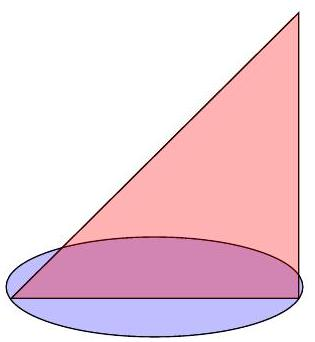
\includegraphics[max width=\textwidth, center]{2024_12_27_3b8e65ac2e3b34a6249eg-4}
\end{enumerate}

Figure 1: A cross section of $S$ depicted in red

Show that the volume of $S$ is

$$
V=\frac{8}{3} r^{3}
$$

\section*{Solution:}
In order to find the volume, we centre the circle of radius $r$ on the $x y$-plane such that the cross-sections along the $x$-axis are isosceles right triangles. The volume is then

$$
V=\int_{-r}^{r} A(x) \mathrm{d} x
$$

where $A(x)$ is the area of the cross section at a fixed value of $x$. Observe that at $x$, the corresponding positive $y$ value is $\sqrt{r^{2}-x^{2}}$. Hence, the length of on side of the triangle is $2 \sqrt{r^{2}-x^{2}}$.\\
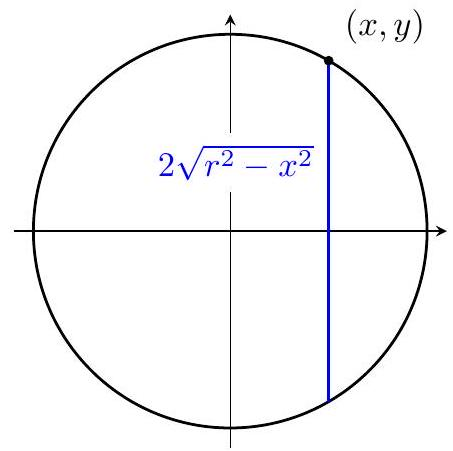
\includegraphics[max width=\textwidth, center]{2024_12_27_3b8e65ac2e3b34a6249eg-4(1)}

The height of the triangle is therefore also $2 \sqrt{r^{2}-x^{2}}$ since we have an isosceles right triangles. Therefore,

$$
A(x)=\frac{1}{2}\left(2 \sqrt{r^{2}-x^{2}}\right)^{2}=r^{2}-x^{2}
$$

We conclude that the volume is

$$
V=\int_{-r}^{r} A(x) \mathrm{d} x=2 \int_{-r}^{r}\left(r^{2}-x^{2}\right) \mathrm{d} x=2\left[r^{2} x-\frac{x^{3}}{3}\right]_{-r}^{r}=\frac{8}{3} r^{3}
$$

Page 5\\
4. Consider the following problems on volumes of revolution using disks/washers.\\
(a) Find the volume of the object created by rotating the region trapped between $f(x)=x-x^{3}$ and $y=0$ about the $x$-axis.\\
(b) Find the volume of the object created by rotating the region trapped between $y=x, x=0$ and $y=3$ about the $y$-axis.\\
(c) Find the volume of the object created by rotating the region trapped between $y=(x-$ $2)^{2}, y=0$ and $x=1$ about the the line $x=1$.\\
(d) Find the volume of the object created by rotating the region trapped between $y=$ $\cos (x), y=-\cos (x)$ which contains the origin about the the line $y=-1$.

\section*{Solutions:}
(a) Notice first that $f(x)=x-x^{3}$ meets the line $y=0$ at $x=0$ and at $x=1$. Thus, in the region trapped between $x-x^{3}$ and $y=0, x$ ranges from 0 to 1 . Now, notice that the area of the region can be evaluated by integrating with respect to $x$. One can imagine that we are "adding up" infinitely many vertical segments. Rotating one of the vertical segment at $x$ about the $x$-axis, we obtain a disk. These disks are precisely the cross-sections of the object.\\
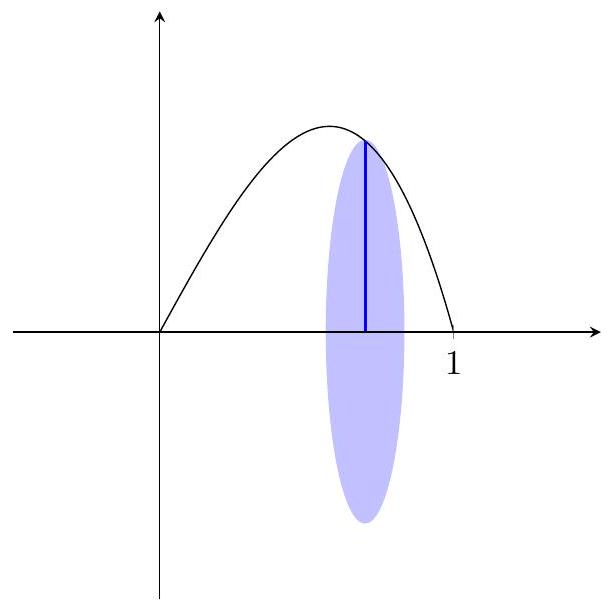
\includegraphics[max width=\textwidth, center]{2024_12_27_3b8e65ac2e3b34a6249eg-6}

Now, the radius of each disk is $r(x)=x-x^{3}$. Thus, the area is

$$
A(x)=\pi(r(x))^{2}=\pi\left(x-x^{3}\right)^{2}=\pi\left(x^{2}-2 x^{4}+x^{6}\right) .
$$

Ergo, the volume of the region rotated about the $x$-axis is

$$
V=\int_{0}^{1} A(x) \mathrm{d} x=\pi \int_{0}^{1}\left(x^{2}-2 x^{4}+x^{6}\right) \mathrm{d} x=\pi\left[\frac{x^{3}}{3}-\frac{2 x^{5}}{5}+\frac{x^{7}}{7}\right]_{0}^{1}=\frac{8}{105} \pi
$$

(b) The region trapped between $y=x, x=0$ and $y=3$ is a triangle. One can evaluate the area by integrating with respect to $y$ from $y=0$ to $y=3$. We can imagine that we are "adding up" infinitely many horizontal segments. For a fixed $y$, rotating one of these segments about the $y$-axis yields a disk which corresponds to the cross-section of the solid of revolution.\\
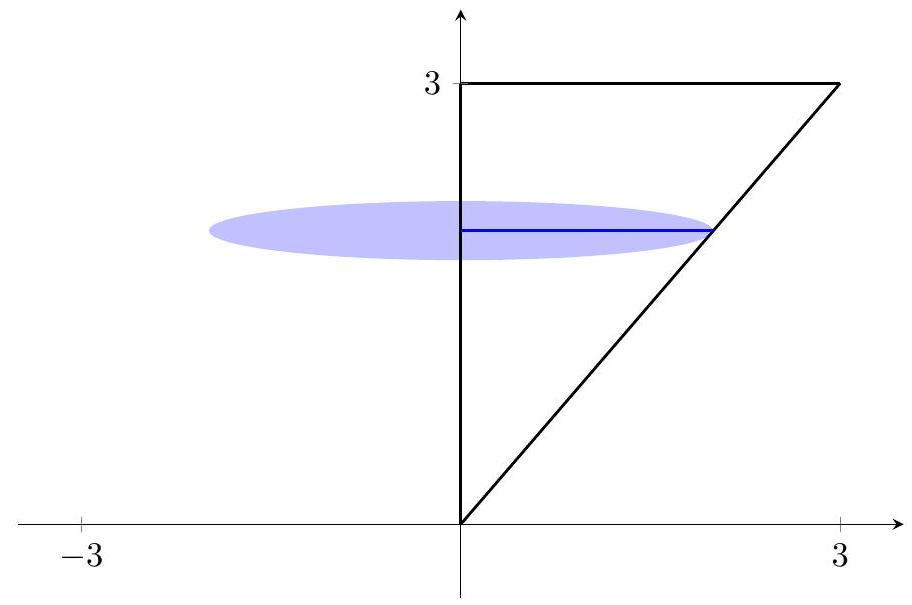
\includegraphics[max width=\textwidth, center]{2024_12_27_3b8e65ac2e3b34a6249eg-7}

Observe that, with respect to $y$, the radius of this disk is $r(y)=y$. Hence, the area of the disk is

$$
A(x)=\pi(r(y))^{2}=\pi y^{2}
$$

Ergo, the volume of the region rotated about the $y$-axis is

$$
V=\int_{0}^{3} A(y) \mathrm{d} y=\pi \int_{0}^{3} y^{2} \mathrm{~d} y=\pi\left[\frac{y^{3}}{3}\right]_{0}^{3}=9 \pi
$$

(c) Note first that, for $x \leq 2$, the curve $y=(x-2)^{2}$ corresponds to $x=2-\sqrt{y}$. Therefore, the region that we will rotate is enclosed by $x=2-\sqrt{y}, y=0$ and $x=1$. The area of this region can be evaluated by integrating with respect to $y$ from 0 to 1 . At a given $y$, we imagine one of the horizontal segments that contributes to the area. Rotating this segment about $x=1$ yields a disk which corresponds to the cross-section of the solid of revolution. The radius of this disk is $r(y)=(2-\sqrt{y})-1=1-\sqrt{y}$. Hence, the area of the disk is

$$
A(x)=\pi(r(y))^{2}=\pi(1-\sqrt{y})^{2}=\pi(1-2 \sqrt{y}+y)
$$

Therefore, the volume of our object is

$$
V=\int_{0}^{1} A(y) \mathrm{d} y=\pi \int_{0}^{1}(1-2 \sqrt{y}+y) \mathrm{d} y=\pi\left[y-\frac{4}{3} y^{3 / 2}+\frac{1}{2} y^{2}\right]_{0}^{1}=\frac{\pi}{6}
$$

(d) Notice that $y=\cos (x)$ intersects $y=-\cos (x)$ precisely when $\cos (x)=0$. In other words, when $x=\frac{\pi}{2}+k \pi$ for some integer $k$. Thus, in the region enclosed between these curves which contains the origin, the $x$ value ranges from $-\frac{\pi}{2}$ to $\frac{\pi}{2}$. The area of this region can be obtained by integrating with respect to $x$. At a given point $x$, we can imagine one of the vertical segments that "add up" to the area. Rotating one of these segments about $y=-1$ yields a washer (i.e. the difference of two disks). This washer is a cross-section of the solid of revolution. The outer radius is

$$
R(x)=\cos (x)-(-1)=\cos (x)+1
$$

The inner radius is

$$
r(x)=-\cos (x)-(-1)=1-\cos (x)
$$

Hence, the area of the washer is

$$
A(x)=\pi(R(x))^{2}-\pi(r(x))^{2}=\pi\left((\cos (x)+1)^{2}-(1-\cos (x))^{2}\right)=4 \pi \cos (x)
$$

Hence, the volume of the enclosed region rotated about $y=-1$ is

$$
V=\int_{-\pi / 2}^{\pi / 2} A(x) \mathrm{d} x=4 \pi \int_{-\pi / 2}^{\pi / 2} \cos (x) \mathrm{d} x=\left.4 \pi \sin (x)\right|_{-\pi / 2} ^{\pi / 2}=8 \pi
$$


\end{document}